% Befehl \fibelkwentry: Ein Eintrag für das Kreuzworträtsel. Vgl. auch Artikel
% „Persoenlichkeitsentwicklung.tex“.
%	Parameter #1: Nummer
%	Parameter #2: Hinweis
\newcommand{\fibelkwentry}[2]{
	% Text um die Breite der Nummerierung einrücken
	\settowidth{\hangindent}{000~}
	% Verhindern, dass innherhalb eines Absatzes auf eine neue Spalte oder
	% Seite umgebrochen wird
	\interlinepenalty=10000
	\makebox[\widthof{000~}][r]{#1~}\ignorespaces#2%
}

\section[Kreuzworträtsel]{}
% brauchen mehr Platz auf der Seite
\enlargethispage{10pt}
\vspace{-1.8cm}
\begin{multicols*}{3}
{% Kein Abstand zw. Paragraphen; linksbündig; kleine Schriftgröße
\parskip=0cm
\RaggedRight
\small

\fibelkwentry{1}{Form des wissenschaftlichen Unterrichts an Hochschulen}

\fibelkwentry{2}{Gegenteil von "fern"}

\fibelkwentry{3}{chem.\ Symbol: Gallium}

\fibelkwentry{4}{Fragewort}

\fibelkwentry{5}{Aufzeichnung hist.\ Ereignisse}

\fibelkwentry{6}{Autor von "Per Anhalter durch die Galaxis"}

\fibelkwentry{7}{Maßeinheit für die Temperatur}

\fibelkwentry{8}{französischer Artikel (f.)}

\fibelkwentry{9}{Abk.: Allgemeiner Studierendenausschuss}

\fibelkwentry{10}{Gebäude des Studierendensekretariats}

\fibelkwentry{11}{Monat}

\fibelkwentry{12}{Maßeinheit für die Zeit}

\fibelkwentry{13}{schnell}

\fibelkwentry{14}{Medium des Lichts?}

\fibelkwentry{15}{Europäische Gemeinschaft}

\fibelkwentry{16}{Heimatuni: \_\_\_\_ Mater}

\fibelkwentry{17}{Segelfliegen: Luftströmung}

\fibelkwentry{18}{Erregung}

\fibelkwentry{19}{nicht Mikro, sondern\dots}

\fibelkwentry{20}{lat.: ich}

\fibelkwentry{21}{engl.: wählen (Telefon)}

\fibelkwentry{22}{erleuchten}

\fibelkwentry{23}{Hersteller von Videospielen}

\fibelkwentry{24}{Zeitmessgerät}

\fibelkwentry{25}{König, Kaiser}

\fibelkwentry{26}{veraltete Einheit des Drucks}

\fibelkwentry{27}{Produkt des Huhns}

\fibelkwentry{28}{bayr.\ Fluss}

\fibelkwentry{29}{Abk.: Papierchromatographie/ Physikalische Chemie}

\fibelkwentry{30}{Bezeichnung für Temperatur}

\fibelkwentry{31}{Einheit für Widerstände}

\fibelkwentry{32}{Heiligenbild}

\fibelkwentry{33}{griech. Buchstabe}

\fibelkwentry{34}{Abk.: experimentell}

\fibelkwentry{35}{chem.\ Symbol für Zirkonium}

\fibelkwentry{36}{Quotient aus Kraft und Fläche}

\fibelkwentry{37}{übellaunig, wohl oder übel}

\fibelkwentry{38}{nichts Neues, nur \dots}

\fibelkwentry{39}{Beate \dots}

\fibelkwentry{40}{Kellner}

\fibelkwentry{41}{Kurzname für Ulrich}

\fibelkwentry{42}{senkrecht auf einer Ebene stehende Gerade}

\fibelkwentry{43}{geschlossen}

\fibelkwentry{44}{Masseneinheit}

\fibelkwentry{45}{chem.\ Symbol für ein Edelgas}

\fibelkwentry{46}{frz.: in}

\fibelkwentry{47}{feuchter Schnee}

\fibelkwentry{48}{dort}

\fibelkwentry{49}{Wertpapier}

\fibelkwentry{50}{Lithium}

\fibelkwentry{51}{griech.: Fertigkeit}

\fibelkwentry{52}{Frucht}

\fibelkwentry{53}{Pointe}

\fibelkwentry{54}{Abk.: Trinitrotoluol}

\fibelkwentry{55}{Abk.: Arbeitskreis}

\fibelkwentry{56}{Vorsilbe: Stern\dots}

\fibelkwentry{57}{engl.: Ende}

\fibelkwentry{58}{Erfolg, "Treffer"}

\fibelkwentry{59}{Kuhantilope der afrikanischen Steppgebiete}

\fibelkwentry{60}{Mühlenabfall von Getreide}

\fibelkwentry{61}{Lehre von den Eigenschaften bewegter Flüssigkeiten}

\fibelkwentry{62}{\_\_posant}

\fibelkwentry{63}{Freundlichkeit}

\fibelkwentry{64}{lat.\ Vorsilbe: weg-, ent-}

\fibelkwentry{65}{Abk.: Vereinte Nationen}

\fibelkwentry{66}{Thermodynamik: "Linie, auf der das Volumen konstant ist"}

\fibelkwentry{67}{kühles Genussmittel aus Milch}

\fibelkwentry{68}{chem. Symbol für Schwefel}

\fibelkwentry{69}{Zahl}

\fibelkwentry{70}{engl.: er}

\fibelkwentry{71}{Institutsgruppe (Abk.)}

\fibelkwentry{72}{Menschenmenge}

\fibelkwentry{73}{Bankrott}

\fibelkwentry{74}{Annahme: \_\_\_\_ung}

\fibelkwentry{75}{Beat}

\fibelkwentry{76}{weibl. Vorname: \dots\ Basinger}

\fibelkwentry{77}{gefärbte Flüssigkeit für Füllfederhalter}

\fibelkwentry{78}{frz.: verkaufen}

\fibelkwentry{79}{große Anzahl}

\fibelkwentry{80}{Dreiländer\dots}

\fibelkwentry{81}{Nationalitätenkennzeichen von Schweden}

\fibelkwentry{82}{Zeit, in der die Hälfte der Atomkerne zerfällt}

\fibelkwentry{83}{Schauspieler: Robert\dots}

\fibelkwentry{84}{moralisch}

\fibelkwentry{85}{Personalpronomen (2.~P.\ Sg.)}

\fibelkwentry{86}{engl.: "mich"}

\fibelkwentry{87}{Abk.: Knockout}

\fibelkwentry{88}{Konjunktionswort}

\fibelkwentry{89}{Mannschaft}

\fibelkwentry{90}{\dots, Mond und Sterne}

\fibelkwentry{91}{frz.: Anfang}

\fibelkwentry{92}{mit zwei Aspekten, doppelt}

\fibelkwentry{93}{Gesangsgruppe}

\fibelkwentry{94}{Chemie: Bezeichnung für kolloide Lösungen}

\fibelkwentry{95}{Abk.: Europäische Union}

\fibelkwentry{96}{Einheit der Kraft}

\fibelkwentry{97}{InterCity}

\fibelkwentry{98}{engl.: es}

\fibelkwentry{99}{geflochtene Einkaufstasche aus Weiden}

\fibelkwentry{100}{Technische Hochschule}

\fibelkwentry{101}{Moderichtung}

\fibelkwentry{102}{Kapitän der Enterprise}

\fibelkwentry{103}{griech.\ Buchstabe}

\fibelkwentry{104}{engl.: alt}

\fibelkwentry{105}{engl.: neu}

\fibelkwentry{106}{Schelm}

\fibelkwentry{107}{Außerirdisches Wesen}

\fibelkwentry{108}{Durcheinander}

\fibelkwentry{109}{Tonstufe}

\fibelkwentry{110}{Zuflucht, Unterkunft}

\fibelkwentry{111}{chem.\ Zeichen für Barium}

\fibelkwentry{112}{Lichtquant}

\fibelkwentry{113}{Spanien}

\fibelkwentry{114}{frz. Artikel}

\fibelkwentry{115}{engl.: Lied}

\fibelkwentry{116}{Zustimmungswort}

\fibelkwentry{117}{Sektart, ital.\ Provinz}

\fibelkwentry{118}{Kohlenstoff}

\fibelkwentry{119}{"Studentenrestaurant"}

\fibelkwentry{120}{Kfz-Zeichen für Münster}

\fibelkwentry{121}{lat.\ Vorsilbe: zu-, hin-, an-}

\fibelkwentry{122}{sich im Rhythmus bewegen (Nomen)}

\fibelkwentry{123}{Autokennzeichen für Steinfurt}

\fibelkwentry{124}{Wildkatze}

\fibelkwentry{125}{organische Derivate des Ammoniaks (Einzahl)}

\fibelkwentry{126}{Familienbund}

\fibelkwentry{127}{feucht, nass}

\fibelkwentry{128}{Modifikation des Sauerstoffs}

\fibelkwentry{129}{Zahl}

\fibelkwentry{130}{The Original Series}

\fibelkwentry{131}{Minerale, milchig-weiße Edelsteine}

\fibelkwentry{132}{Verkehrsfunk-Automatik}

\fibelkwentry{133}{engl.: ja}

\fibelkwentry{134}{überhöhte Antwort eines schwingungsfähigen Systems auf äußere Anregung}

\fibelkwentry{135}{lat.: ich bin}

\fibelkwentry{136}{österr. Komponist (\dag~1809)}

\fibelkwentry{137}{Geschmacksorgan}

\fibelkwentry{138}{Bez.\ für die kleinstmögliche., unteilbare Einheit jeder Energieform}

\fibelkwentry{139}{Not, Missstand}

\fibelkwentry{140}{Würde}

\fibelkwentry{141}{chem.\ Symbol für Stickstoff}

\fibelkwentry{142}{span.: Insel}

\fibelkwentry{143}{Nationalitätenkennzeichen der Niederlande}

\fibelkwentry{144}{Version von Windows}

\fibelkwentry{145}{kein Wert}

\fibelkwentry{146}{kein Wert}
}

\fibelsig{Judith, Niki}
\end{multicols*}

% Textbereich der Seite etwas vergrößern, damit mehr Bild reinpasst
\enlargethispage{\baselineskip}
\begin{center}
	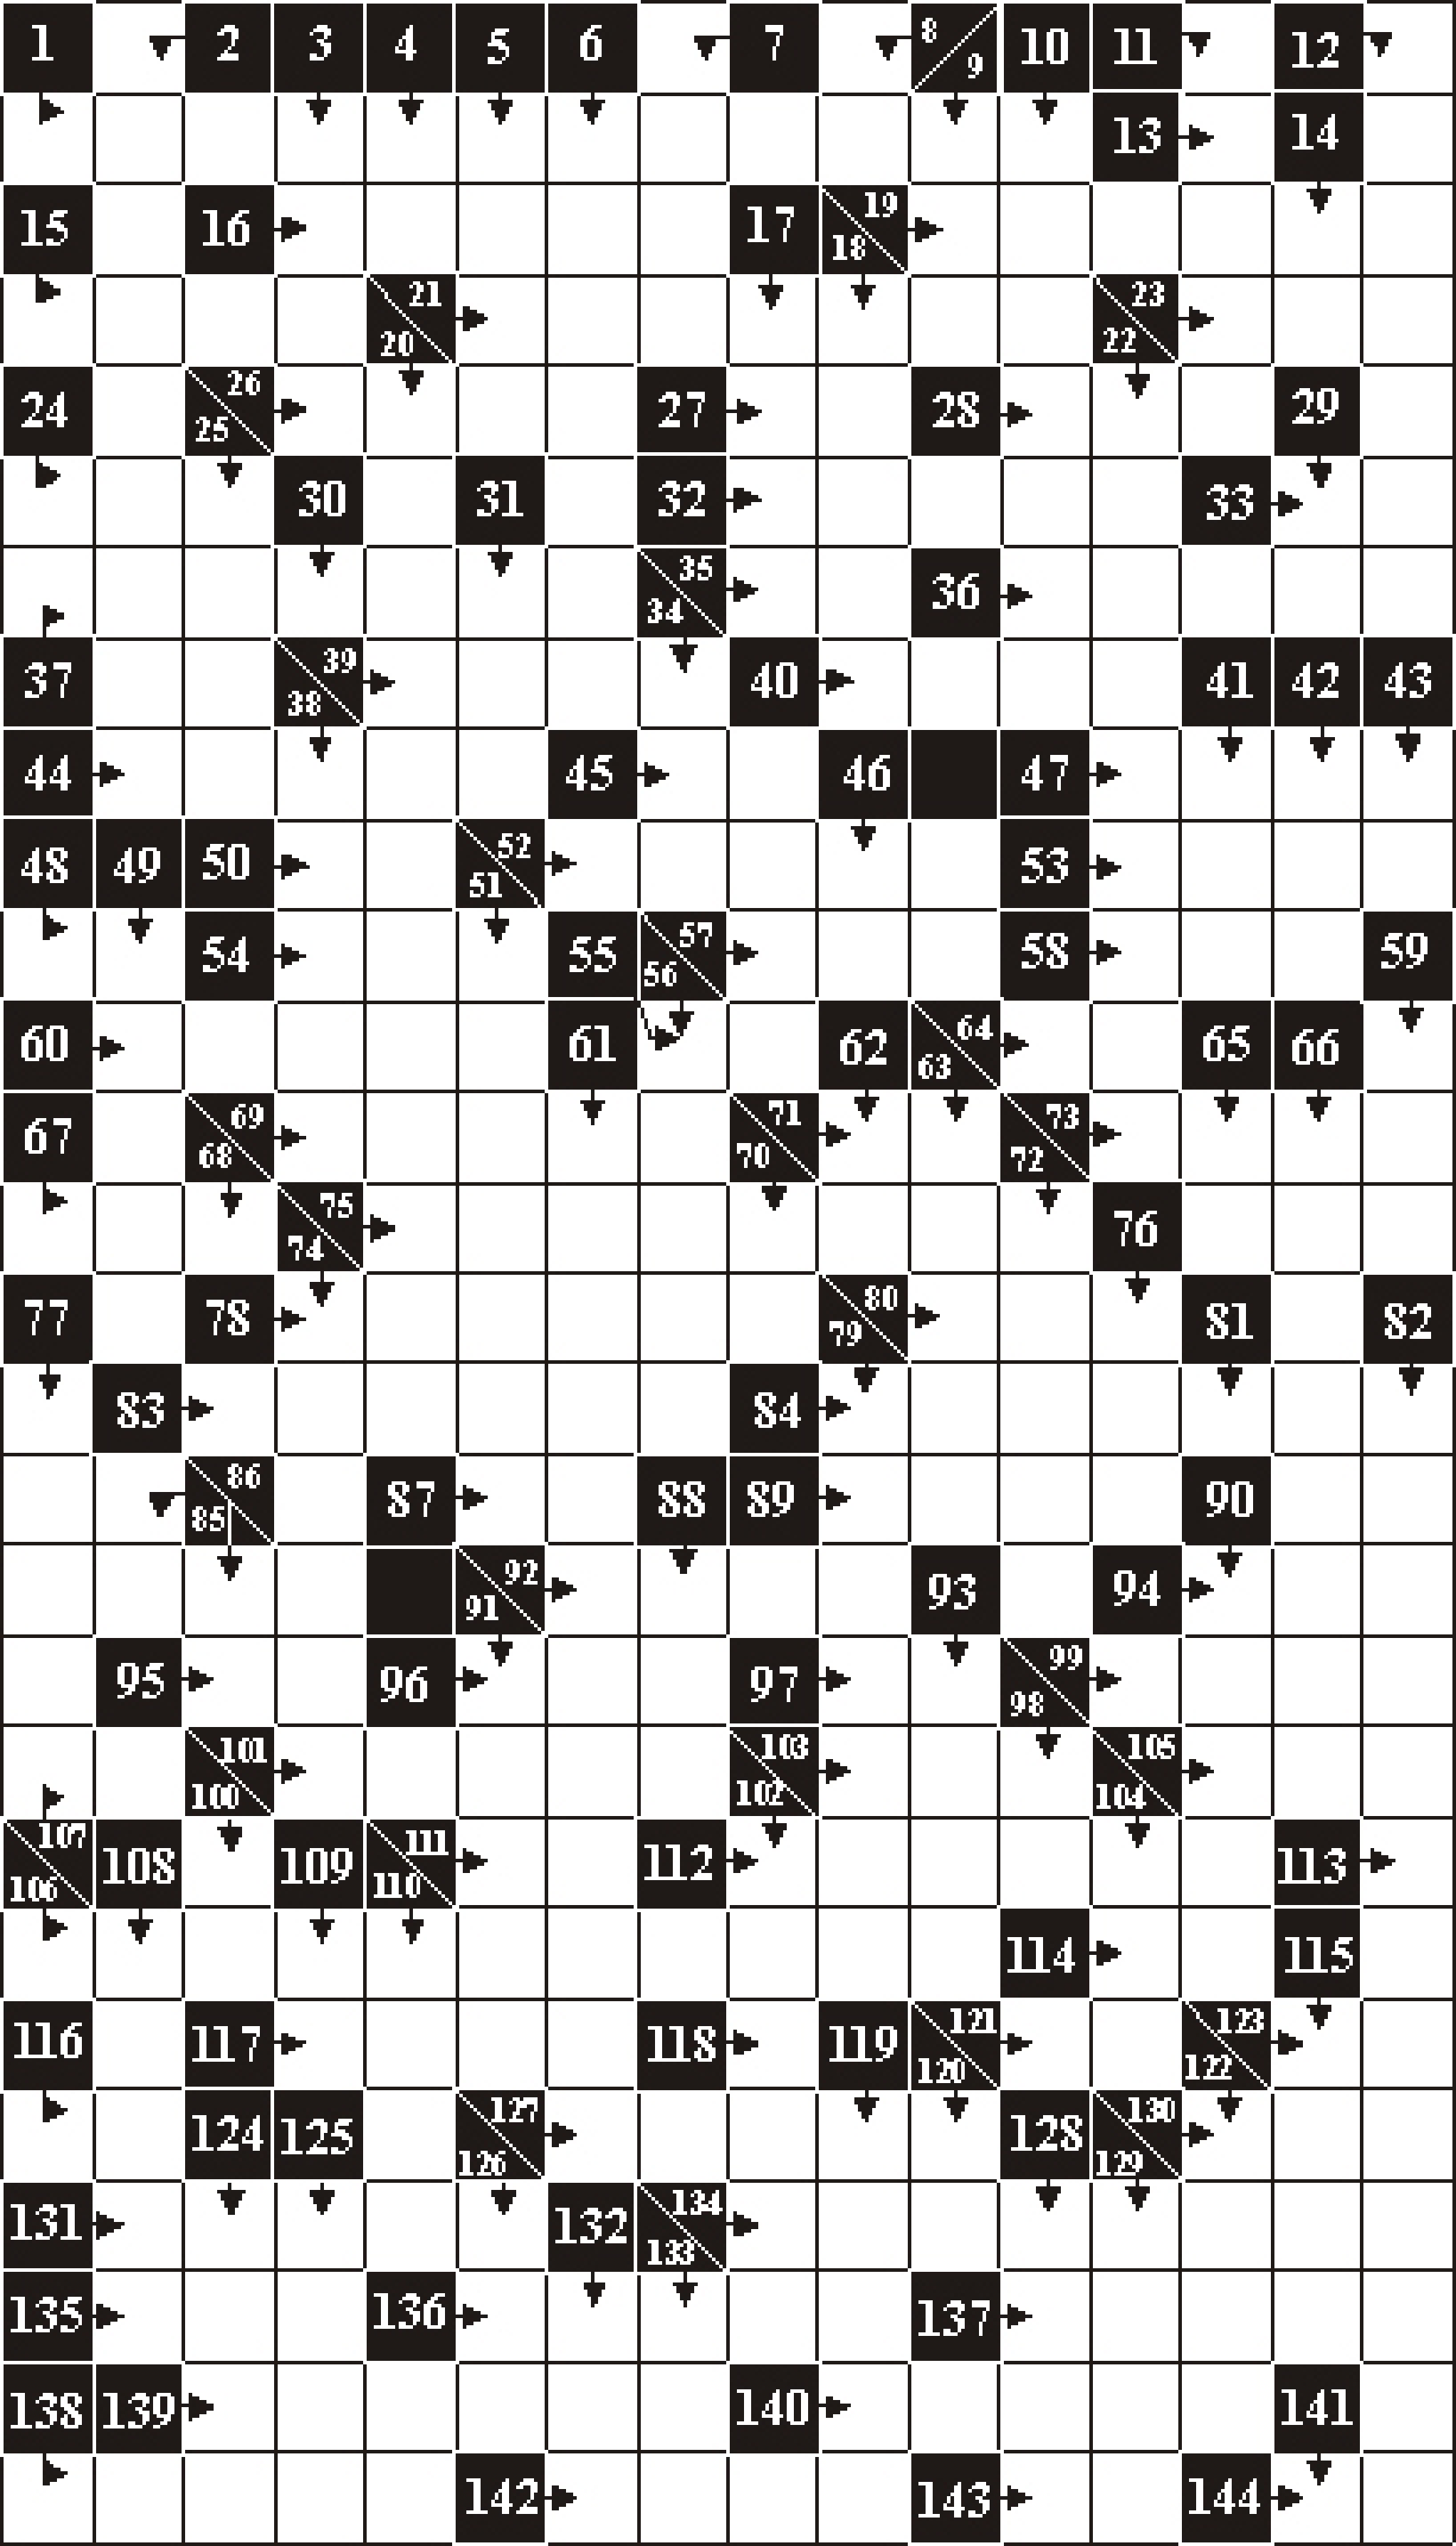
\includegraphics[height=\textheight]{res/kreuzwortraetsel_hires.png}
\end{center}
